\chapter{Influence du l'approximation de vitesse de la lumière réduite sur la propagation de l'ionisation}
\label{sec:intre:zreio}

%%%%%%%%%%%%%%%%%%%%%%%%%%%%%%%%%%%%%%%%%%%%%%%%%%%%%%%%%%%%%%%%%%%%%%%%%%%%%%%%%%%%%%%%%%%%%%%%%%%%%%%%%%%%%%%%%%%%%%%%%%%%%%%%%%%%%%%%%%%%%%%%%%%%%%%%%%%%%%%%%%%%%%%%
%%%%%%%%%%%%%%%%%%%%%%%%%%%%%%%%%%%%%%%%%%%%%%%%%%%%%%%%%%%%%%%%%%%%%%%%%%%%%%%%%%%%%%%%%%%%%%%%%%%%%%%%%%%%%%%%%%%%%%%%%%%%%%%%%%%%%%%%%%%%%%%%%%%%%%%%%%%%%%%%%%%%%%%%
%%%%%%%%%%%%%%%%%%%%%%%%%%%%%%%%%%%%%%%%%%%%%%%%%%%%%%%%%%%%%%%%%%%%%%%%%%%%%%%%%%%%%%%%%%%%%%%%%%%%%%%%%%%%%%%%%%%%%%%%%%%%%%%%%%%%%%%%%%%%%%%%%%%%%%%%%%%%%%%%%%%%%%%%

%\chapter{Vitesse de la lumière réduite et vitesse des fronts d'ionisation.}
%\label{sec:lightspeed}

%Nous verrons finalement l’application de cette méthode sur la quantification de l’approximation de la vitesse de la lumière réduite (\ac{RSLA})
%Comme abordé dans la section \ref{sec:rad_solver}, le calcul de la radiation est coûteux en terme de ressources.
%Ceci car la condition de Courant impose d'exécuter un grand nombre de pas de temps pour suivre correctement l'évolution d'un processus très rapide sur une durée déterminée.
%L'idée de la \ac{RSLA} est que la vitesse de la lumière est significativement plus rapide que la vitesse des autres processus à l’œuvre dans la simulation.
%Partant de ce constat, même en la réduisant, cette vitesse devrait rester significativement supérieure, et mener aux même résultats.
%En divisant la vitesse par un facteur donné, on peux augmenter la taille du pas de temps de ce même facteur, et donc diminuer le nombre total de pas de temps total à exécuter, et donc le coût global du solveur radiatif.
%Nous avons déjà abordé le sujet de la \ac{RSLA} et j'invite le lecteur à se référer à la section \ref{sec:RSLA} pour plus de détails.

%Une des variables que l'on cherche a reproduire dans les simulations de l'\ac{EoR} est l'état d'ionisation de l'\ac{IGM} à la fin de la réionisation.
%La raison principale est qu'il existe des contraintes observationnelles sur cet état (voir section \ref{sec_contraintes_obs}).
%Un des objectifs des simulations numérique de l'\ac{EoR} est, à partir de ces contraintes observationnelles, d'estimer toute l'histoire d'ionisation de l'Univers.
%Nous allons pour cela utiliser les cartes de redshift de réionisation, qui contiennent pour chaque point de l'espace, le redshift auquel il a été ionisée.
%Ce type de carte, contient énormément d'information sur l'histoire d'ionisation du volume simulé et en font un outils important pour l'étude de la réionisation dans son ensemble.



Nous avons abordé dans la partie précédente une étude centrée sur les halos, représentatifs des régions de hautes densités. %sur-denses et contenant la plus grande partie de la masse.
Nous nous intéressons dans cette section à un aspect complémentaire, l'état d'ionisation de l'\ac{IGM}, qui lui est représentatif de la plus grande partie du volume.

Cette section fait référence au travail en cours présenté en annexe\,\ref{pap:c}, et on cherche ici a étudier l’évolution de la fraction ionisée en analysant l'évolution des bulles ionisées.
Cette étude se base sur les cartes de redshift de réionisation, un outil qui permet de condenser toute l'histoire d'ionisation d'une simulation.
A partir de cet outil, il est possible de quantifier la vitesse à laquelle les fronts d'ionisation se propage dans l'\ac{IGM}.

Dans ce chapitre, l'objectif est d'explorer l'impact de la \ac{RSLA} (voir section \ref{sec:RSLA}), sur la propagation de l'ionisation dans les simulations.
La \ac{RSLA} permettant d'obtenir des gains substantiels au niveau du coût de calcul de la radiation \citep{rosdahl_ramsesrt_2013, aubert_radiative_2008, 2001NewA....6..437G}, il est essentiel de quantifier dans quelle mesure cette approximation est correcte.
%J'ai comparé une série de simulations identiques à l'exception de la vitesse de la lumière réduite et observé que cette dernière a un impact sur l'histoire de réionisation.
Je présenterai comment j'ai implémenté le calcul des cartes de redshift de réionisation à la volée dans EMMA ainsi qu'une méthode de calcul de la vitesse des fronts d'ionisation.
Cette méthode sera ensuite appliquée à une série de simulations avec différentes \ac{RSLA}.
Nous verrons que dans nos modèles la réionisation est un processus qui s’exécute en deux phases et que en fonction de la \ac{RSLA} l'une ou l'autre est impactée.
%On cherche également à déterminer dans quelle mesure notre interprétation des résultats doit être révisée si cet impact est conséquent.

% j'ai utilisé l'outil développé dans la section précédente pour comparer une série de simulations identiques à l'exception de la vitesse de la lumière réduite (voir section \ref{sec:RSLA}).

%
%Je présenterai ensuite une méthode pour déterminer la vitesse des fronts d’ionisations à l'aide de ces cartes.
%Nous verrons finalement grâce à ces carte que la réionisation est un processus qui s'effectue en deux temps, le second étant un emballement qui va "flasher" le volume.


%Nous avons vu que la réionisation est un processus qui s'effectue en deux phases, et nous verrons ici que en fonction de la \ac{RSLA}, l'une ou l'autre est affectée.


\section{Calcul des cartes de redshift de réionisation}
\label{sec:zmapcompute}

Les carte de redshift de réionisation ont été introduite par \cite{2008ApJ...689L..81T} et sont des outils contenant une l'information du déroulement de la réionisation d'une manière extrêmement compacte.
Nous allons voir dans cette section comment elles sont calculées.

En première approximation, il est possible de considérer l'état d'ionisation comme binaire.
La fraction ionisée évoluant très rapidement en présence de rayonnement, l'\ac{IGM} est soit presque exclusivement neutre soit presque exclusivement ionisé (voir figure \ref{fig:xionmap}).
Ceci est dû au fait qu'à nos résolutions les gradients d'ionisation au niveau des fronts ne sont faiblement résolus voir pas du tout.
En gardant l'information du passage entre ces deux états, il est possible de créer une carte, en 3 dimensions, contenant l’information de toute l'histoire d'ionisation de l'\ac{IGM}.


\begin{figure}
        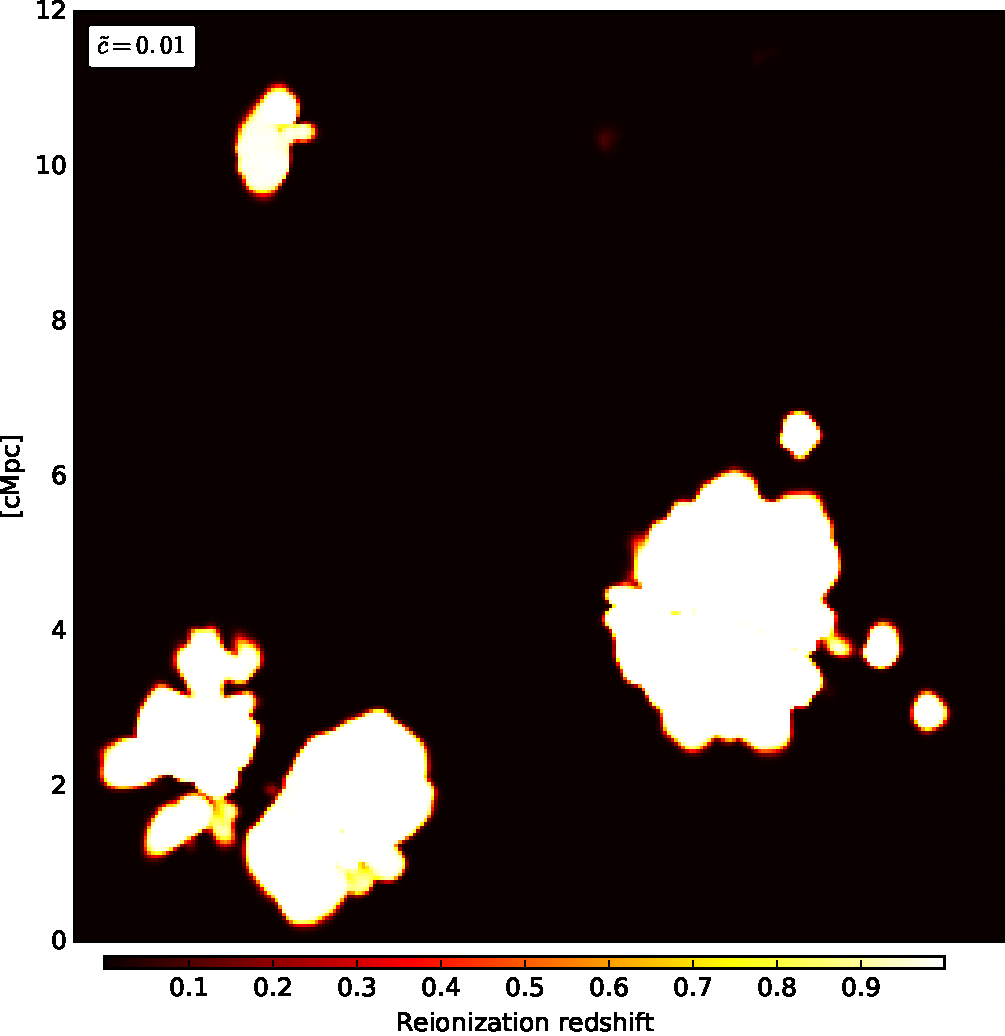
\includegraphics[width=.95\linewidth]{img/04_mapreio/xion_map.pdf} 
        \caption[Carte d'ionisation]{Exemple de carte d'ionisation à $z=10$.
        En première approximation, l'état d'ionisation est binaire, ionisé autour des sources et neutre loin de celles ci.
 		\label{fig:xionmap}}
\end{figure}

L'instant à conserver sera défini comme l'instant de passage de la fraction d'ionisation de la cellule par un seuil.
Le passage d'un état à l'autre étant rapide, la valeur de ce seuil a un impact réduit et ce seuil sera définis par la suite à 50\%.
Cette valeur de seuil est régulièrement utilisée dans la litérature \citep{iliev_cosmological_2006, doi:10.1111/j.1365-2966.2011.18219.x, 2012A&A...548A...9C}.
Il s'avère également que c'est le taux d'ionisation considérer dans les études du \ac{CMB} pour déterminer le redshift de réionisation de l'Univers.

Comme certaines des cellules les plus denses peuvent recombiner, il existe deux façons de définir un redshift de réionisation: il est possible de considérer soit la première, soit la dernière ionisation.

\begin{itemize}
\item Dans le cas de la première ionisation, la valeur ne devra être mise à jour qu'une seule fois au moment du passage du seuil.
Pour ce faire, toutes les cellules seront initialisées à une valeur caractéristique (eg -1).
La mise à jour ne se fera donc qu'à la condition que la fraction d'ionisation soit supérieure au seuil et que la valeur actuelle du redshift d'ionisation soit -1.
Ainsi la valeur ne sera pas remise à jour à chaque pas de temps où la cellule sera ionisée. 

\item Dans le cas de la dernière ionisation, la valeur du redshift sera mise à jour, tant que la fraction d'ionisation de la cellule est inférieure au seuil.
Ainsi, si un cellule recombine, le valeur de son redshift associé sera de nouveau mise à jour, et la mise à jour stoppera à chaque passage au dessus du seuil.
\end{itemize}

Il est possible de calculer ces cartes à partir des sorties disques de EMMA mais dans le but d'obtenir la meilleur résolution temporelle possible, j'ai implémenté dans EMMA le calcul des cartes de réionisation à la volée, pendant l'exécution d'une simulation.
Le principe de l'implémentation est présenté sur le listing \ref{lst:majz}.

\begin{lstlisting}[float=bth,language=c,frame=tb,caption={Mise a jour du redshift de reionisation},label=lst:majz]
  #define THRESH_MAP (0.5) // definition du seuil

  // Derniere ionisation 
  if(cell.xion<THRESH_MAP) // test de l'ionisation de la cellule
    cell.t_last_xion=current_t; // association du temps d'ionisation 

  // Premiere ionisation 
  if( (xion>=THRESH_MAP) && (cell.t_first_xion==-1) ) // test de l'ionisation de la cellule et de premiere ionisation
    cell.t_first_xion=current_t; // association du temps d'ionisation 
\end{lstlisting}

%Dans le cas d'une grille \ac{AMR}, l'organisation de la grille est amenée à évoluer.
%La question du raffinement/deraffinement se pose alors.
%Si dans le cas du raffinement, l'injection directe du redshift de la cellule mère ne pose pas de problème particulier, les choses sont différentes lors du déraffinement.
%En effet, dans EMMA, quand une cellule est deraffinée la valeur moyenne des 8 cellules filles est injectée dans la cellule mère (voir \ref{Opérateurs de changement de grilles}).
%Le problème est que les processus physiques qui ont lieu dans la simulation sont calculés par rapport au temps et que les redshift ne sont pas linéaire en temps (voir \ref{sec:friedman}).
%Ainsi les redshift ne doivent pas être moyennés.
%Pour résoudre ce problème, j'ai fait le choix de travailler non pas avec le redshift mais avec l'age de l'Univers au moment de l'ionisation de la cellule.
%Les cartes de temps pourront être converties en cartes de redshift en post traitement, le passage entre ces deux grandeurs étant réalisé par intégration de la cosmologie à l'aide de l'équation \ref{eq:scale_t}.
%Il faudra toutefois prendre garde d'utiliser les mèmes paramètres cosmologiques que ceux utilisés en interne de la simulation.

Un exemple de carte de première réionisation obtenue est présenté sur le figure \ref{fig:zmap}.
%Cette carte a été générée a partir d'une simulation présentant des caractéristiques similaires à celles des simulation présentées au chapitre précédent (voir section \ref{sec:pres_simu}).
%Elle a un volume de $\left( 8h^{-1} \mathrm{cMpc} \right) ^3$ et 
Il s'agit de la même tranche (une cellule d’épaisseur - $45$ ckpc) que celle présentée sur la figure \ref{fig:xionmap}, on y retrouve le contour des bulles à $z=10$.
On y observe différentes zones ionisées à redshift élevé ($z>10$), localisant les sources de radiation et donc les zones de densités élevées.
Autour des sources ce trouve des motifs concentriques, fortement anisotrope, en forme de "papillons".
Il sont dû à la non homogénéité de l'\ac{IGM}, la propagation du rayonnement étant ralentie par la présence de filaments de densité élevée.
Enfin on mesure de grandes étendues ayant un redshift de réionisation similaire ($z<8$), il s'agit des régions sous-denses, où le rayonnement peut se propager quasi librement, et peux donc ioniser un vaste volume dans un intervalle de temps restreint.

\begin{figure}
        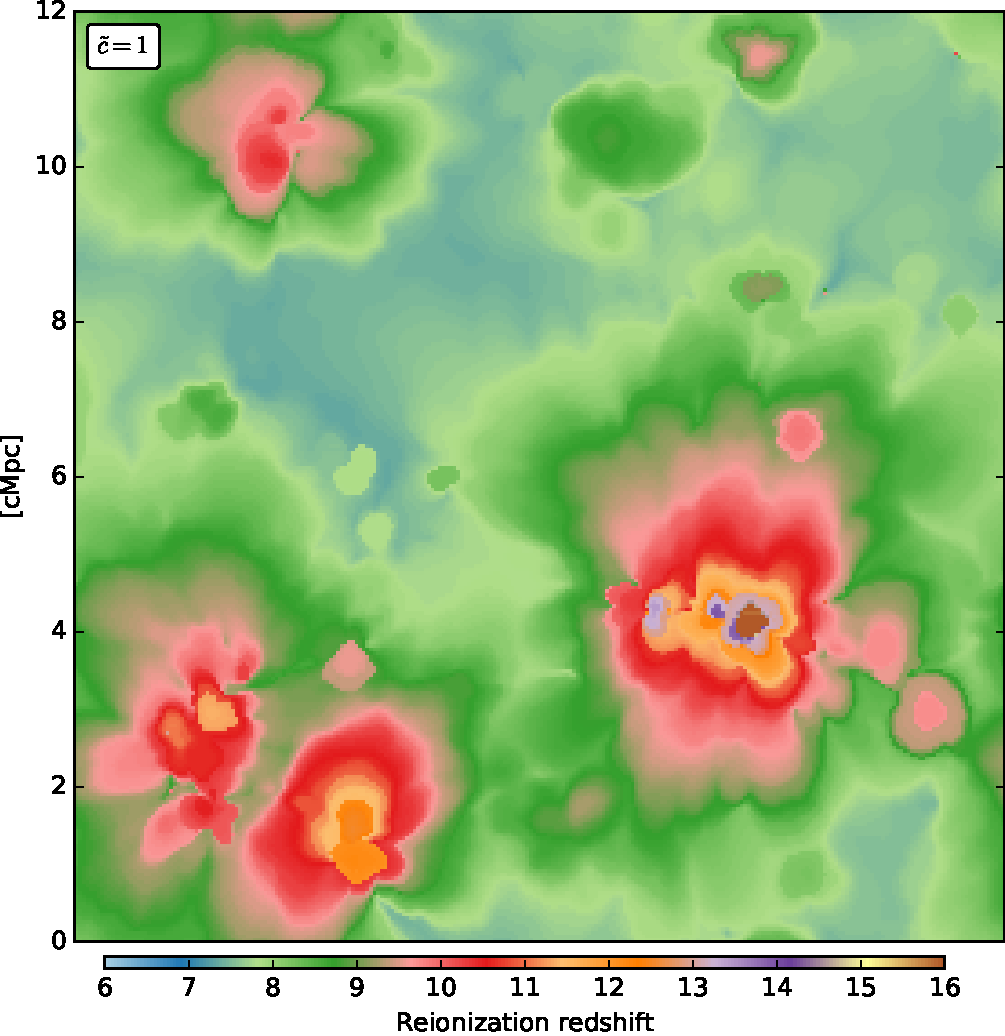
\includegraphics[width=.95\linewidth]{img/04_mapreio/map_z_c1.pdf} 
        \caption[Carte de redshift d'ionisation]{Exemple de carte de redshift d'ionisation générée par EMMA.
        Cette carte contient toute l'histoire de réionisation de la simulation.
        Il s'agit d'une tranche d'une cellule d'épaisseur centrée sur la première cellule ionisée.
 		\label{fig:zmap}}
\end{figure}

D'un point de vue technique, la méthode de calcul des cartes proposée ici se base la grille, et donc sur une représentation Eulérienne, pour stocker les instants de réionisation.
Le problème peut être abordé sous un autre angle en utilisant une carte de réionisation Lagrangienne, se basant sur les particules de matière noire et permettant d'obtenir une information complémentaire à la carte actuelle.
Ce type de carte permettrait d'obtenir l'information de réionisation, instantanément après la recherche de halos, facilitant grandement l'analyse des simulations de grandes tailles similaire à celle que nous traiterons dans le chapitre \ref{sec:z0}.

\section{Calcul de la vitesse des fronts d’ionisation à partir des cartes de redshift}
\label{sec:vreio}

Partant du principe que les cartes de redshift d'ionisation contiennent l'information d'une grande partie de l'évolution de la fraction d'ionisation dans la simulation, il est possible d'en extraire la vitesse de propagation des fronts d'ionisation.
%À partir des cartes de redshift de réionisation
%L'idée est la suivante:
%En utilisant le fait que ces cartes représentent un temps pour chaque point de l'espace, il est possible de déterminer quel est le temps qu'il s'est écouler entre la réionisation de deux cellules adjacentes, et donc de connaître la vitesse à laquelle le front d'ionisation les a traversé.
%En pratique, la vitesse des fronts sera obtenue en calculant le gradient de la carte de réionisation.
%Le gradient représente le temps $dt$ mis par le front pour parcourir une distance $dx$ correspondant à la taille de la cellule.
En utilisant le fait que ces cartes représentent un temps pour chaque point de l'espace, la vitesse des fronts sera obtenue en calculant le gradient de la carte de réionisation.
%Pour obtenir directement une vitesse il est préférable de travailler en temps et non en redshift.
%Or il reste un problème à régler, la carte de vitesse obtenue est en unité comobile, alors que la lumière voyage avec une vitesse physique.
%La carte de vitesses obtenue étant en unités comobile, et l'objectif étant de comparer la vitesse des fronts d'ionisation à la vitesse de la lumière réelle, le gradient sera pondéré par la valeur du facteur d'expansion au moment de l'ionisation de la cellule associée pour travailler en unités physiques.
%On obtiendra ce facteur par intégration de la cosmologie, de la même façon que pour transformer la carte de temps en carte de redshift.
Le gradient sera discrétisé par une différence finie centrée de la manière suivante:

\begin{equation}
\vec{\nabla} t_{reio}^i \approx \frac{t^{i+1}  - t^{i-1}}{2a^i \Delta x }. %\left( x^{i+1}  - x^{i-1} \right)
\end{equation}

ou $i$ est l'indice de la cellule, $a$ le facteur d'expansion, $t$ l'instant d'ionisation et $\Delta x$ la taille des cellules.
On notera que le calcul est effectué sur une carte de temps et non un carte de redshift.

Ce gradient représente le temps nécessaire à l'ionisation d'une certaine distance.
La vitesse des fronts d'ionisation $V_{reio}$ est alors définie comme l'inverse de la norme de ce gradient:

\begin{equation}
V_{reio}  = \left | \frac{1}{ \vec{\nabla} t_{reio}} \right| .
\end{equation}

Par souci de simplicité, et comme le calcul du gradient est problématique au niveau des interfaces entre niveaux de raffinement, les études présentées ici ont été réalisées en projetant la grille \ac{AMR} sur le niveau de base, de manière à n'avoir qu'un seul niveau, et à supprimer ces interfaces.
Un exemple de carte de vitesses de fronts obtenue est présenté sur la panneau supérieur de la figure \ref{fig:vmap}.
Comme sur la figure \ref{fig:zmap}, on y observe des motifs concentriques autour des sources.
Ces motifs sont composés d'une alternance de vitesses lentes et rapides représentant les générations successives d'étoiles.
Lorsque la source centrale d'une bulle ionisée s’éteint, le front d'ionisation ne peut plus progresser et la vitesse diminue.
Dans notre modèle (cf section \ref{sec:etoilerad}) les sources subissent une forte décroissance de luminosité, et le front n'est pas stoppé mais fortement ralenti.
Lorsqu'une (ou plusieurs) nouvelle particule stellaire se forme au sein de la bulle, le front recommence sa progression.
On mesure dans un certain nombre de régions, des anneaux de vitesses faibles ($\approx 10^{-4}$c) ayant une taille caractéristique de quelques centaines de kiloparsec.
Ces anneaux sembles dû à l'extinction de la première génération d'étoile : dans ce cas la formation stellaire au sein du halo n'est pas fortement établie, et il faut un certain temps pour que la génération suivante prenne la relève, la vitesse des front ayant alors le temps de fortement ralentir.
On mesure visuellement que la vitesse a tendance à être plus élevée dans les régions sous-denses.

\begin{figure}
        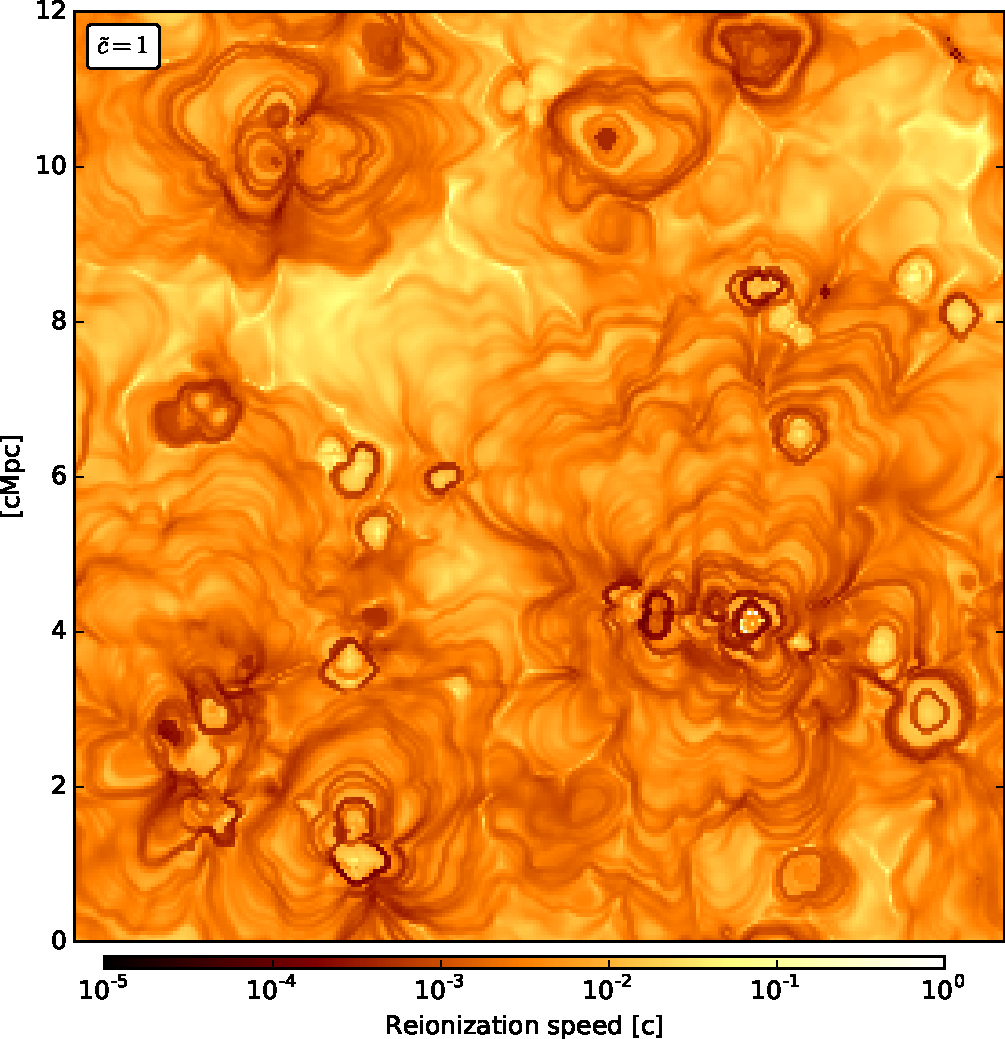
\includegraphics[width=.95\linewidth]{img/04_mapreio/map_v_c1.pdf} 
        
		%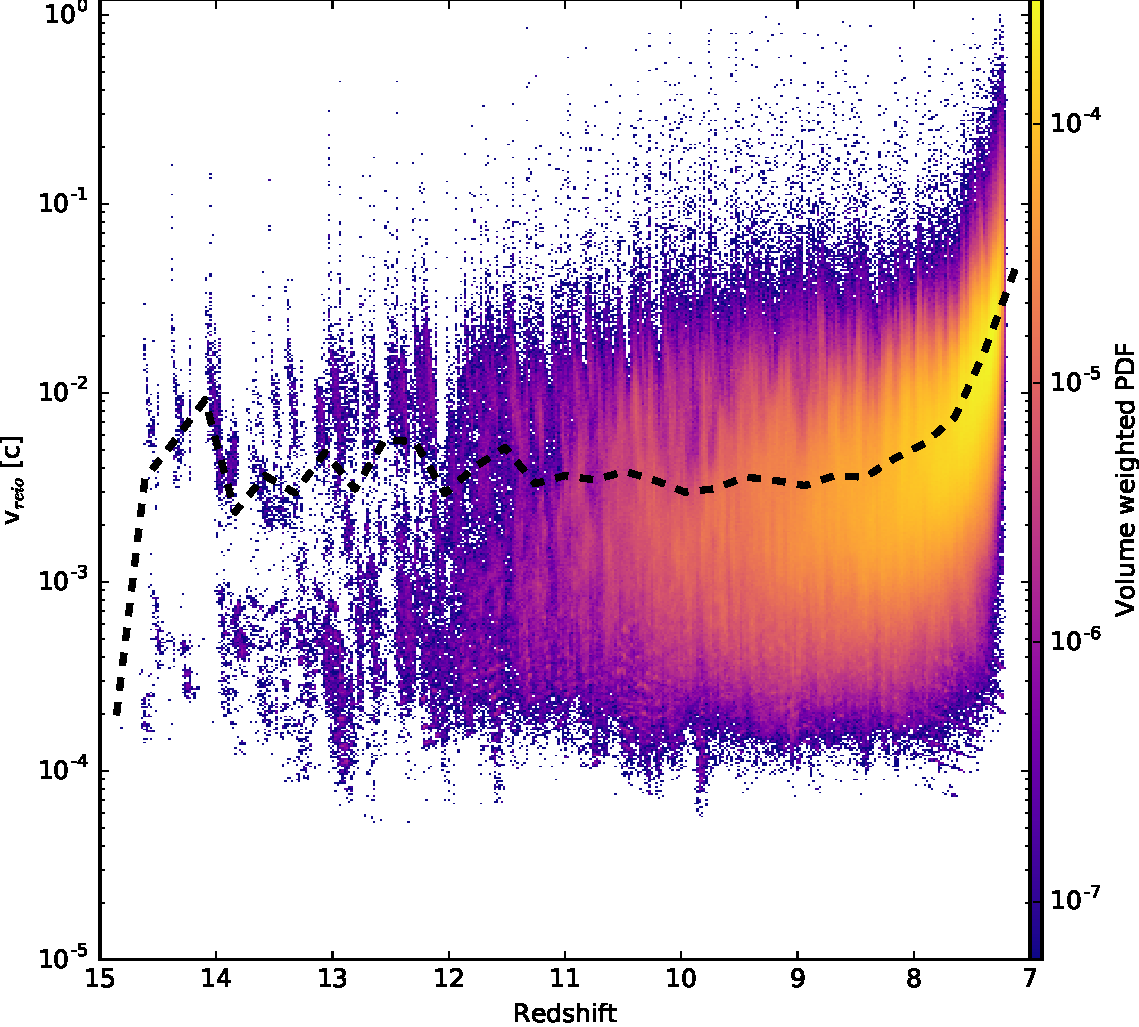
\includegraphics[height=.425\textheight]{img/04_mapreio/speedreio_z.pdf} 
        \caption[Vitesse des fronts d'ionisation]{Vitesse des fronts d'ionisation.
        Haut : exemple de carte de vitesse de fronts générée par la méthode du gradient.
		Cette carte correspond a la même tranche que celle présenté Figure \ref{fig:zmap}
		Bas : vitesse des fronts d'ionisation en fonction du redshift.
        On mesure une accélération des fronts à la fin de la réionisation.
        }
 		\label{fig:vmap}
\end{figure}

Cette méthode peux cependant mener à des valeurs de vitesses aberrantes dans le cas ou deux cellules adjacentes ne se font pas ioniser par la même source.
Ceci peut arriver dans deux cas : 
\begin{itemize}
\item Proche des sources, si deux particules stellaires sont formées en même temps dans deux cellules voisines.
\item Loin des sources, au moment de la rencontre entre deux fronts d'ionisation.
\end{itemize}

Dans ces deux cas il est possible d'avoir deux cellules voisines avec le même redshift d'ionisation. et donc d'obtenir un gradient de temps nul et une vitesse infinie.
En pratique, ces cas extrêmes n'arrivent que rarement avec une probabilité de l'ordre de $10^{-6}$ (quelques cellules dans les simulations considérées).





%\begin{figure}
%        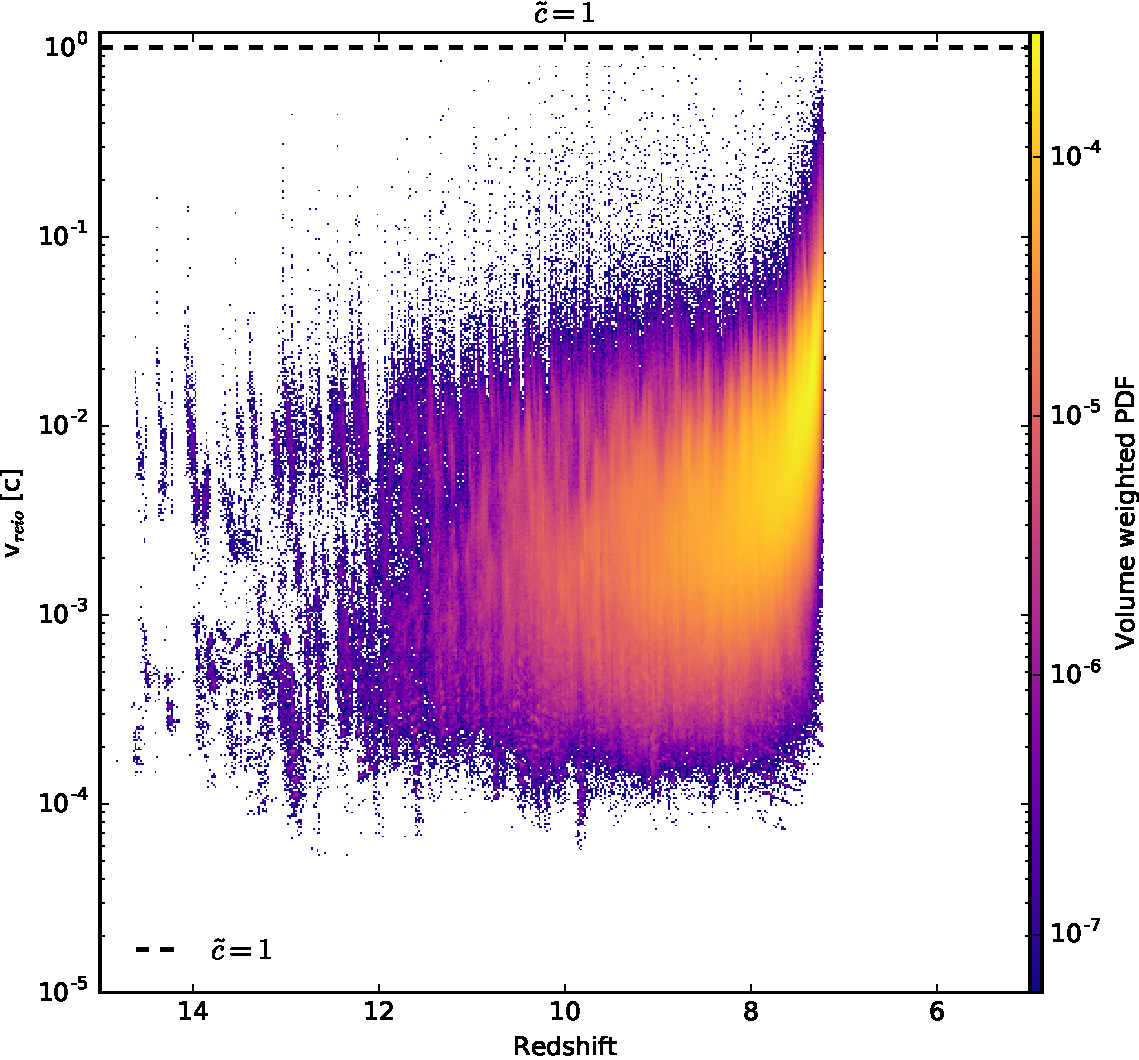
\includegraphics[width=.95\linewidth]{img/04_mapreio/speedreio_z_c1.pdf} 
%        \caption[Évolution de la vitesse des fronts]{Vitesse des fronts d'ionisation en fonction du redshift.
%        On mesure une vive accélération des fronts à la fin de la réionisation.
% 		\label{fig:speedz}}
%\end{figure}


%\clearpage
%\section{Accélération des fronts}
%\label{secaccreio}
%
%De la même manière que lors du calcul de la vitesse, il est possible de dériver une seconde fois la carte de vitesse de front pour obtenir une carte d'accélération des fronts.
%
%
%\subsection{Valeur absolue}
%
%Comme cette seconde dérivation est une dérivation spatiale, l'accélération obtenue est donc une variation spatiale de vitesse (en [m/s/m]).
%Une carte obtenue est présentée sur la figure \ref{fig:accz}.
%On y observe une alternance de phases de faibles et de fortes accélérations.
%Si l'on regarde un film de l'évolution des bulles ionisées, on observe que celle ci progressent par avancées successives
%Lorsque la source centrale d'un halo s’éteint, le front d'ionisation ne peut plus progresser et le front ne peux plus accélérer.
%
%On observe de fortes accélérations proche des sources, la ou la densité de photons est importante.
%Il y a également de fortes accélérations dans les régions sous-denses car la densité d'hydrogène neutre y est faible.
%%Il subit donc une forte décélération.
%%Les valeurs d'accélérations ont tendance a être plus élevée dans les régions sous denses.
%
%\begin{figure}
%        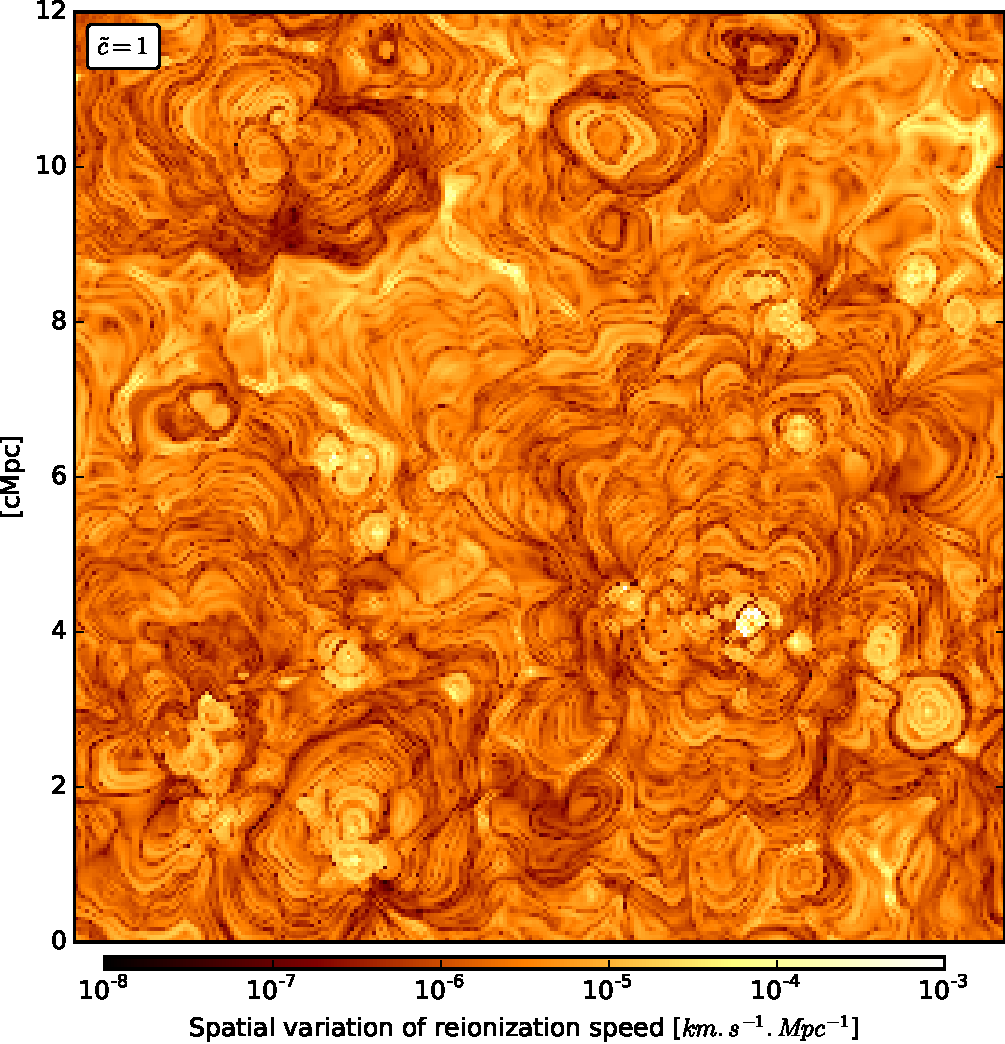
\includegraphics[height=.3\textheight]{img/04_mapreio/map_acc_c1.pdf}\\
%        
%        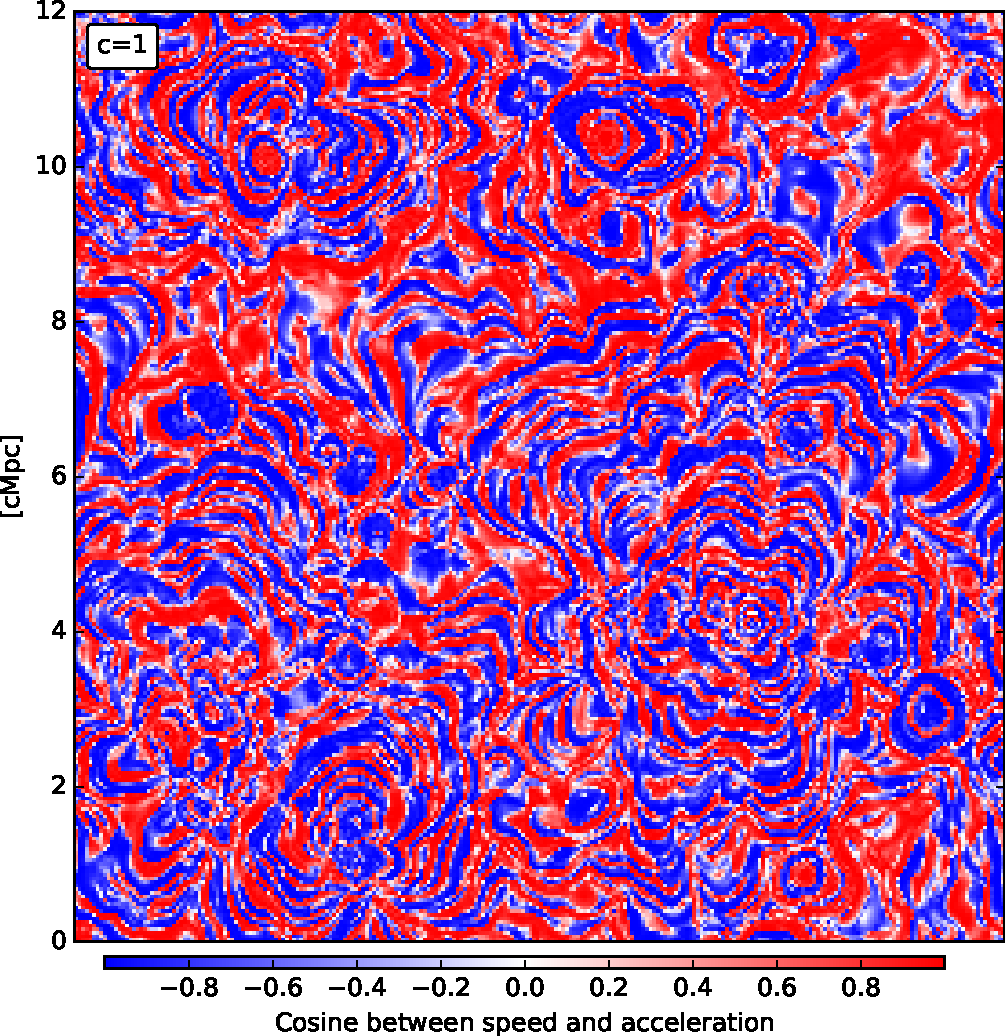
\includegraphics[height=.3\textheight]{img/04_mapreio/map_cos_c1.pdf}
%        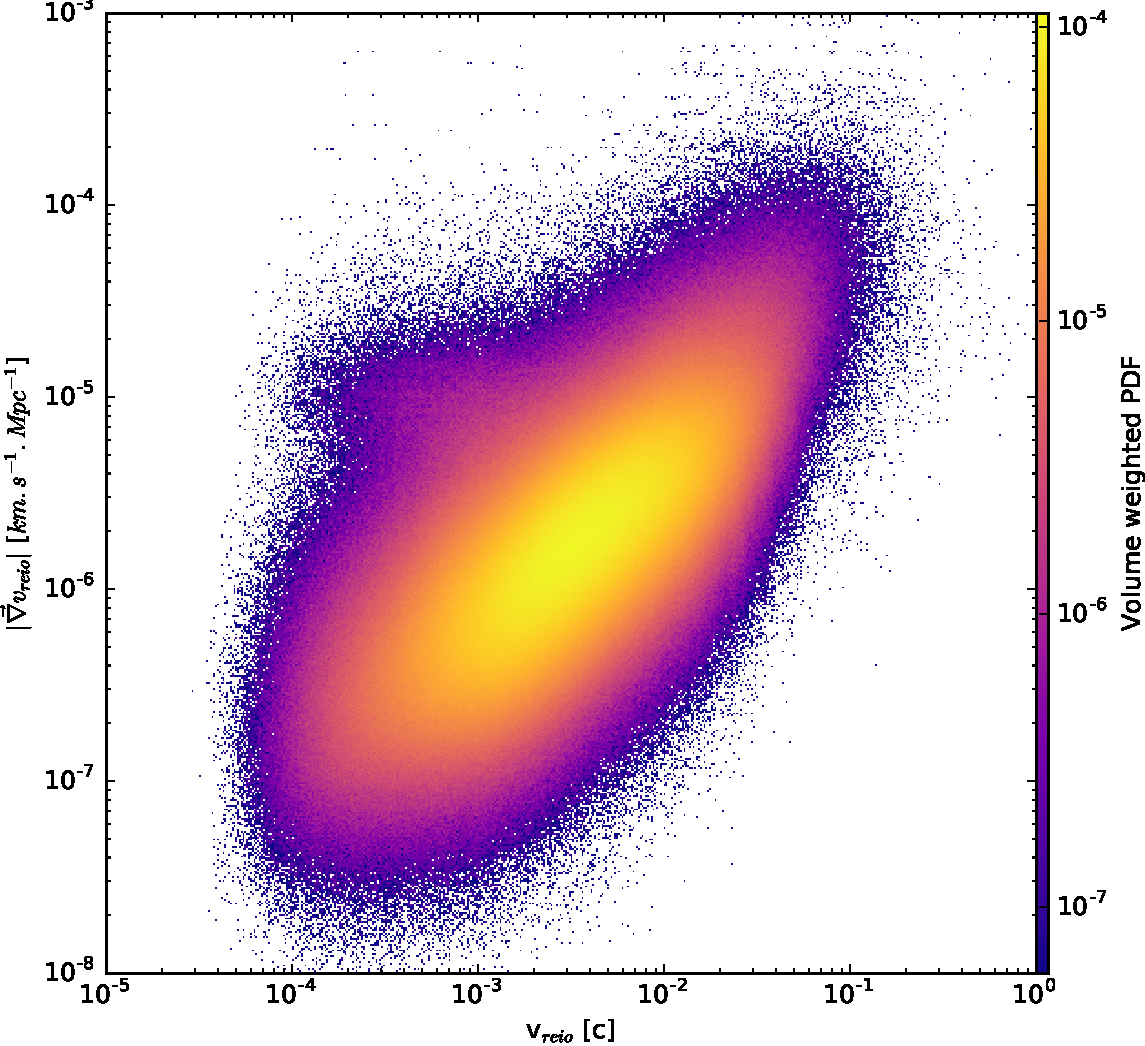
\includegraphics[height=.3\textheight]{img/04_mapreio/v_gradv_c1.pdf} 
%
%        \caption[Accélération des fronts]{Accélération des fronts d'ionisation.
%        Haut : Carte de la valeur absolue de l'accélération.
%%		Les fronts subissent des successions d'accélérations et de décélérations de manière concentrique aux sources.        
%        Milieu : Cosinus de l'angle entre la vitesse et l'accélération.
%%        On observe une alternance de l'angle entre ces deux vecteurs représentative d'une succession d'accélération et de décélération.
%        Bas: Accélération des fronts d'ionisation en fonction de leur vitesse.
%%        Il existe une nette corrélation: plus un front est rapide, plus il accélère.
%%        Les motifs concentriques sont encore accentués.
%        }
% 		\label{fig:accz}
%\end{figure}
%
%
%\subsection{Direction} 
%
%Pour retrouver l'information de la direction de l'accélération des fronts, j'ai calculé l'angle entre la vecteur vitesse des fronts et leur vecteur accélération.
%La carte obtenue est présentée sur la figure \ref{fig:accz}.
%On observe que les vecteurs ont une forte tendance à être alignés ou anti alignés (il y a très peu e blanc sur la figure).
%En effet quand une région HII dispose d'une source de rayonnement suffisamment intense, le front avance radialement à cette source, mais lorsque  en fin de vie cette source s'éteint le front cesse de progresser et décélère fortement.
%
%%\begin{figure}
%%        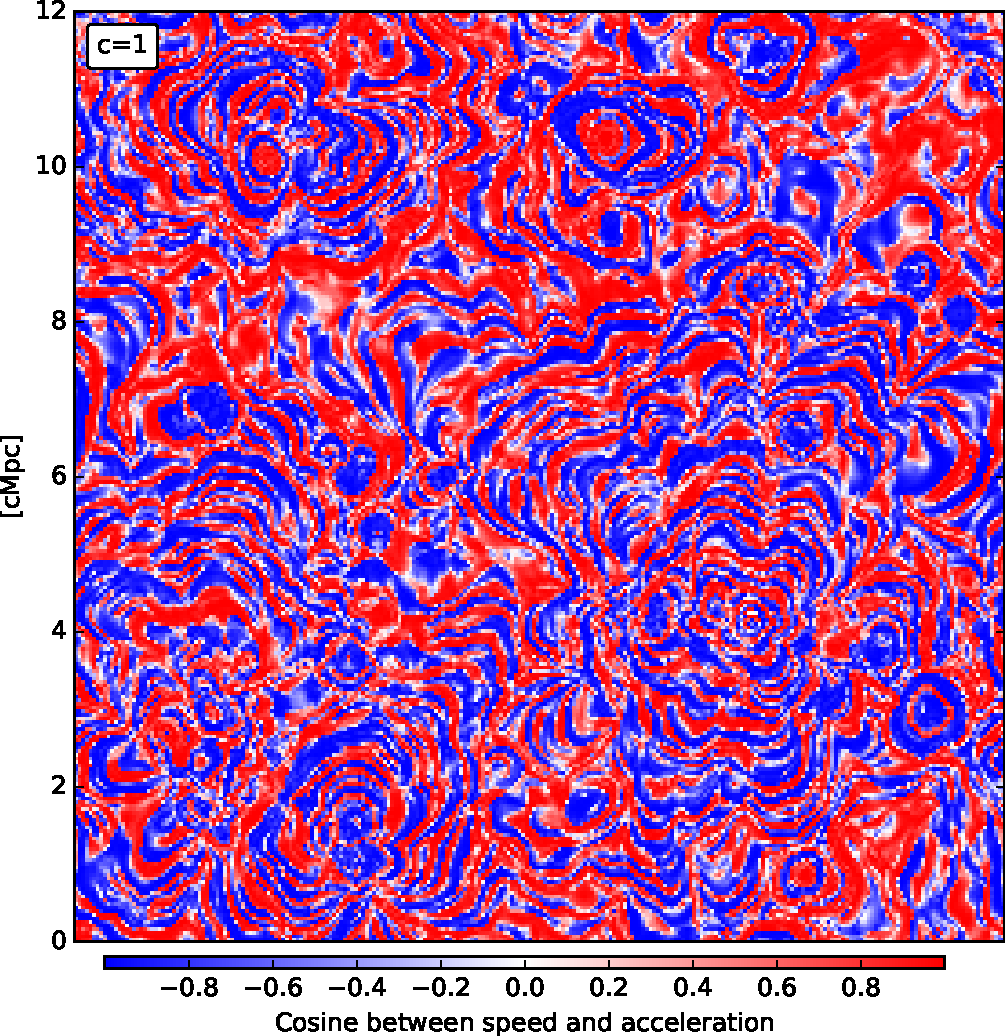
\includegraphics[width=.95\linewidth]{img/04_mapreio/map_cos_c1.pdf} 
%%        \caption[Évolution de l'accélération des fronts]{
%%\label{fig:cos}}
%%\end{figure}
%
%%Ces phases sont liée au temps de vie des sources
%
%%TODO decrire la carte
%
%\subsection{Accélération en fonction de la vitesse}
%
%De la même manière que précédemment, il est possible de lier les cartes de vitesses et d'accélération : figure \ref{fig:accspeed}.
%On y observe que plus un front est rapide, plus il accélère.
%Ce qui conforte l'idée que la réionisation est un processus qui s'emballe.
%On observe également une "bosse", dont je n'ai pas réussi à identifier l'origine.
%
%%\begin{figure}
%%        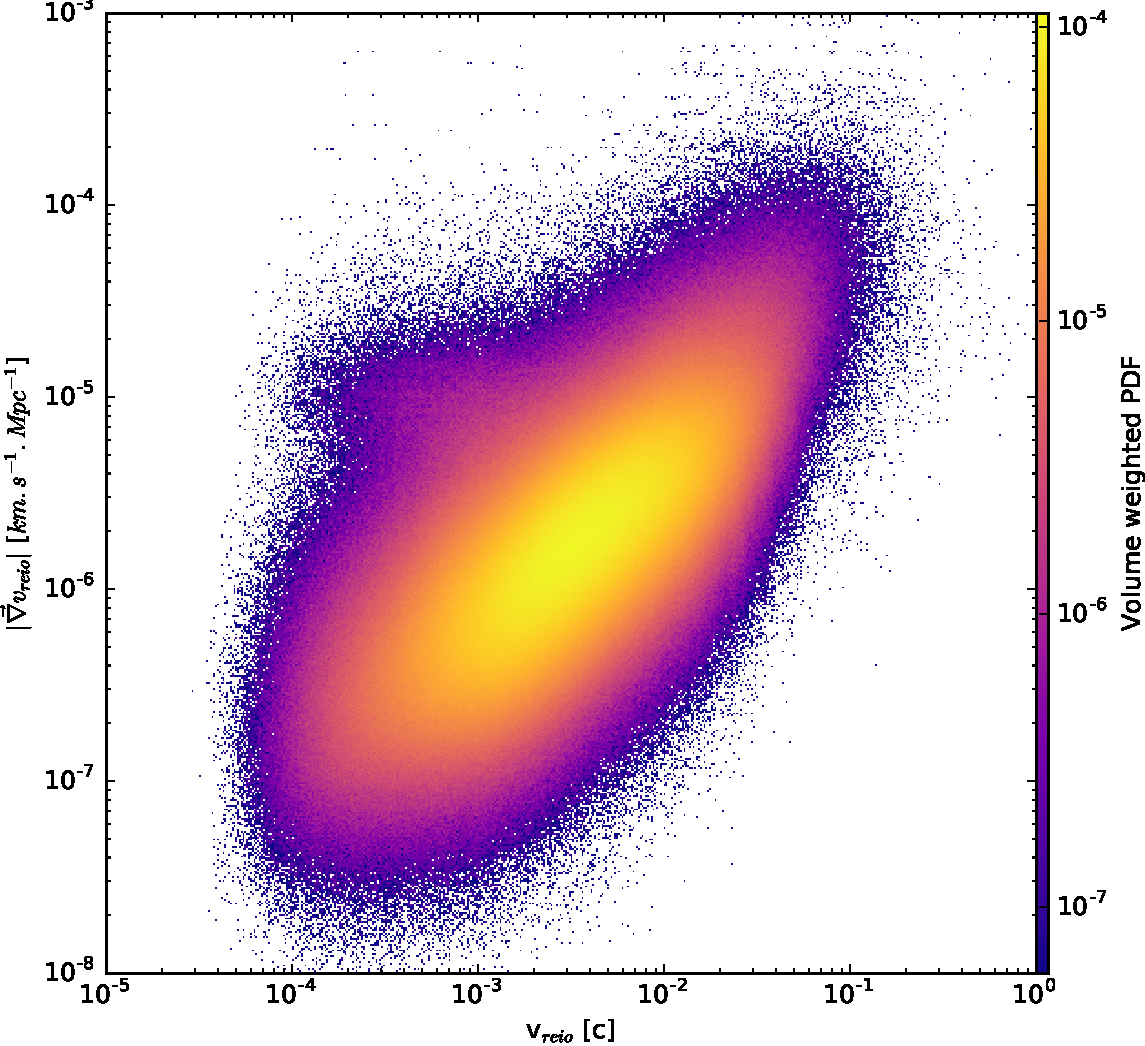
\includegraphics[width=.95\linewidth]{img/04_mapreio/v_gradv_c1.pdf} 
%%        \caption[Évolution de l'accélération des fronts]{Accélération des fronts d'ionisation en fonction de leur vitesse.
%%        Il existe une nette corrélation: plus un front est rapide, plus il accélère.
%% 		\label{fig:accspeed}}
%%\end{figure}
%
%
%
%%\subsection{Vitesse des fronts en fonction du redshift}
%%
%%% \ref{sec:compfrontspeep}
%%


\section{Présentation des simulations}

Les simulations utilisées ici ont des caractéristiques identiques à celles présentées en section \ref{sec:pres_simu}.
Elles ont une taille de $\left( 8 \cdot h^{-1} \mathrm{cMpc } \right)^3$, sont résolues avec $256^3$ éléments et 3 niveaux de raffinements sont autorisés.
Elles ne contiennent pas de supernovæ pour faciliter l'interprétation et minimiser les effets de couplage entre les différentes physiques.
J'ai réalisé six de ces simulations avec des \ac{RSLA} allant de $\tilde{c}=1$ à $\tilde{c}=0.01$.

La \ac{SFH} cosmique et l'histoire d'ionisation de ces six simulations sont présentées sur la figure \ref{fig:zrsla}.
On observe sur le premier panneau de la figure \ref{fig:zrsla} que la \ac{RSLA} n'a pas d'impact sur la \ac{SFH} cosmique, ce qui induit que le budget de photon n'est pas modifié entre les simulations.
Cependant, on mesure sur le second panneau que les histoires d'ionisation sont significativement différentes.% en fonction des \ac{RSLA}.
La \ac{RSLA} a une influence sur la propagation de l'ionisation : plus la vitesse de la lumière est élevée dans la simulation, plus le volume réionise rapidement.
Cet effet a déjà été observé dans des travaux qui utilisent un solveur radiatif utilisant la méthode de moments (eg \cite{rosdahl_ramsesrt_2013}).
On remarquera que pour les courbes des simulations avec $\tilde{c}=0.02$ et $\tilde{c}=0.01$, un retard est pris depuis le début de la réionisation, dans les autres cas, le retard n’apparaît que sur la fin.

On observe également que la fraction de neutre résiduelle est plus élevée lorsque la lumière est plus lente, avec une amplitude allant de $10^{-4}$ à $5 \cdot 10 ^{-5}$.
Par exemple entre la courbe $\tilde{c}=1$ et $\tilde{c}=0.3$ la réionisation à lieu au même moment, mais seule la fraction de neutre résiduelle est impactée.
La vitesse de la lumière réduite intervient dans le calcul de la chimie, et plus particulièrement dans le calcul du taux de photo-ionisation (cf section \ref{sec:chimie}).
Il n'est pas encore clairement établi si la \ac{RSLA} doit s’appliquer à la chimie ou non et cette question mériterait une étude dédiée.
Actuellement, par soucis de cohérence et d'uniformité, la vitesse de la lumière est réduite partout, c'est à dire pour le transport des photons, et dans la gestion de la chimie.
%L'idée est que si les photons sont plus lents, ils mettent plus de temps à parcourir une cellule et disposent donc de plus de temps pour interagir avec le gaz.
%Réduire la vitesse de la lumière dans le module de chimie permet de diminuer le taux de photo-ionisation et en théorie conserver la quantité total d'atomes ionisés.
%De cette manière une vitesse de la lumière plus élevé mènera à une capacité d'ionisation plus grande, mais en contrepartie les photons disposerons de moins de temps pour interagir avec le gaz au sein des cellules.
%La balance semble neutre en théorie mais une fois le volume réionisé, la radiation devient uniforme et le transport n'a plus d’influence.
De ce fait, le taux de photo-ionisation $\Gamma = c \sigma n_\gamma$ augmente avec la vitesse de la lumière et la fraction de neutre résiduelle diminue.

%Ceci est certainement dû au fait que la lumière dispose de plus de temps pour interagir avec le gaz au sein des cellules.

%Sur le troisième volet de la figure \ref{fig:zrsla} est représenté le redshift de réionisation de la boite.
%Ce redshift est définis comme étant le redshift auquel la fraction de neutre de la boite devient inférieur à $10^-{4}$.
%On observe une certaine saturation vers les valeurs s'approchant de $\tilde{c}=1$ et une rapide croissance du redshift de réionisation quand la \ac{RSLA} diminue.
%La saturation des redshifts de réionisation pour les hautes vitesses de la lumière réduite constitue un argument en faveur des techniques de lancé de rayons utilisant une vitesse de la lumière infinie.

%Cependant cette saturation peut également être représentative d'un volume simulé trop petit. 
%En effet \cite{2017arXiv170804238R} estime le libre parcours moyen des photons à la fin de la réionisation à redshift $z\approx 6$ à environ 10 Mpc physique.
%Dans notre cas le volume simulé représente un cube de $\approx 1,7$ Mpc physique.
%Dans de telles conditions, une source peut virtuellement se voir elle même et contribuer à ioniser le milieu 

\begin{figure}
        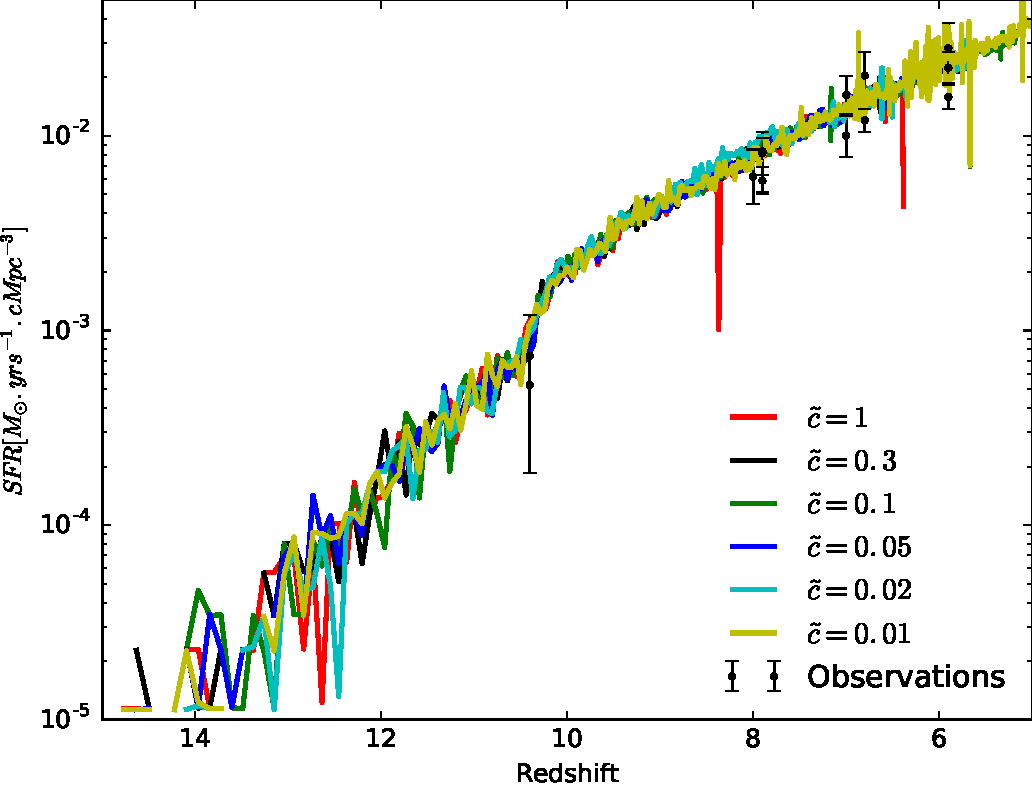
\includegraphics[height=.3\textheight]{img/04_mapreio/SFR.pdf} 
        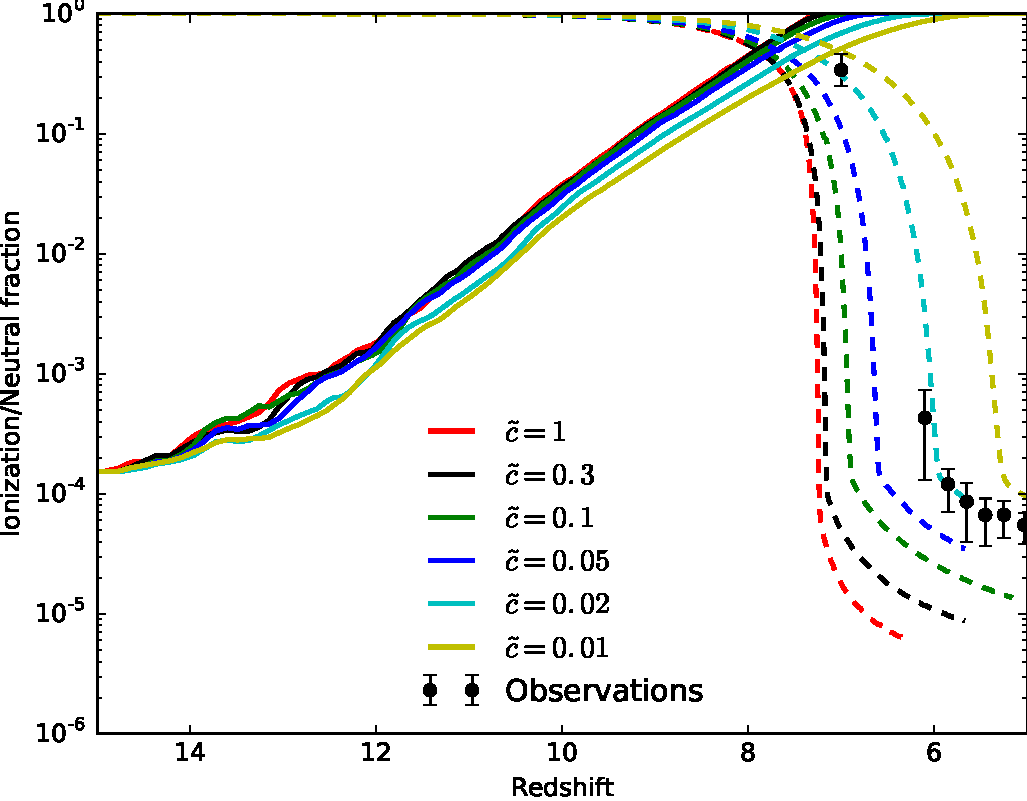
\includegraphics[height=.3\textheight]{img/04_mapreio/xion.pdf} 
%        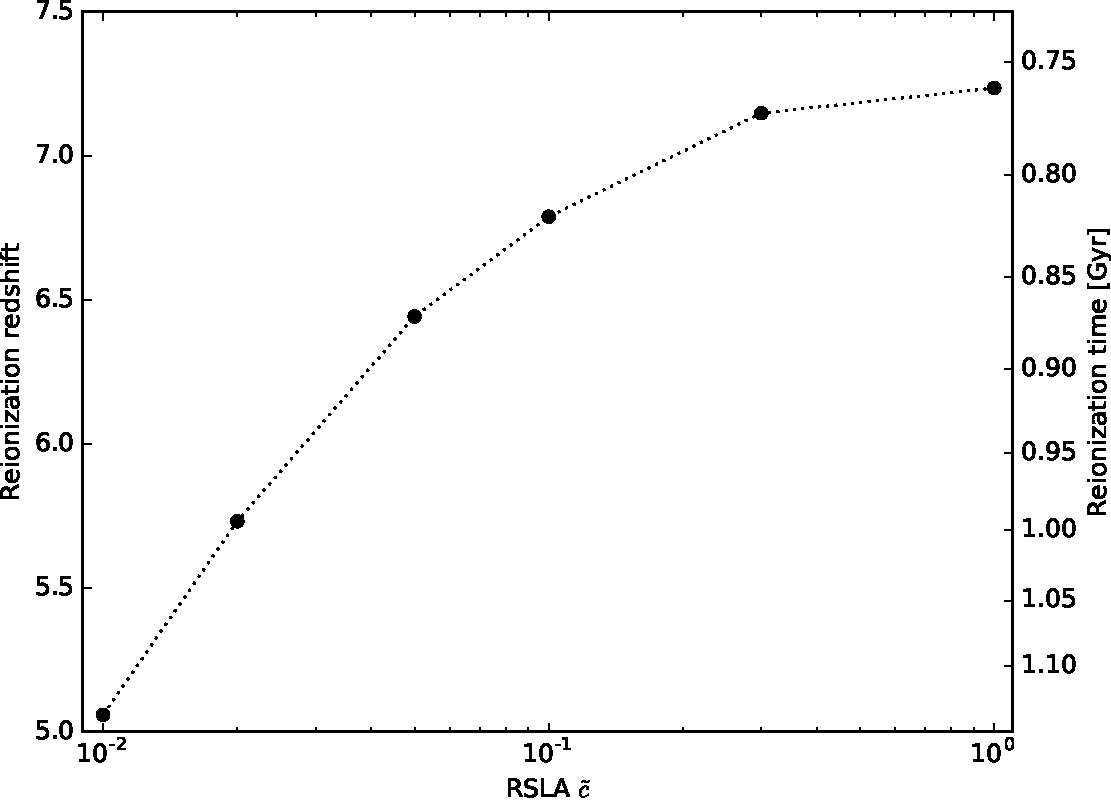
\includegraphics[height=.3\textheight]{img/04_mapreio/z_rsla.pdf} 
        \caption[Redshift de réionisation en fonction de la RSLA]{
		Panneau supérieur: \ac{SFH} en fonction de la \ac{RSLA}.
		La \ac{RSLA} n'influence pas la formation stellaire et le budget de photon.
		Panneau inférieur: histoire d'ionisation en fonction de la \ac{RSLA}.
		La \ac{RSLA} influence fortement l'histoire d'ionisation, une vitesse de la lumière réduite plus faible induit un retard dans la réionisation.
%		Panneau inférieur: redshift de réionisation en fonction de la \ac{RSLA}, une vitesse de la lumière réduite plus faible induit un retard dans la réionisation.
 		\label{fig:zrsla}}
\end{figure}




%Cette histoire est contenue dans un outils essentiel de l'étude de la réionisation dans son ensemble, les cartes de redshift d'ionisation.
%Ces cartes sont constituées en chaque point de l'espace, du redshift auquel chaque cellule est passée au dessus d'un certain niveau d'ionisation moyen.
%Les cartes de redshift de réionisation sont de outils important pour l'étude de la réionisation dans son ensemble.

% et donc 
%Cependant ne sont pas basées sur les halos mais sur l'\ac{IGM}, (voir \ref{sec_contraintes_obs}) et donc sur les régions sous-dense loin des halos.


\section{Évolution de la vitesse des fronts en fonction de la vitesse de la lumière réduite}
\label{sec:compfrontspeep}

Dans les sections \ref{sec:zmapcompute} et \ref{sec:vreio}, nous avons associé à chaque cellule un redshift d'ionisation et une vitesse de front.
En utilisant la méthode du gradient pour calculer la vitesses des fronts d'ionisation en fonction du redshift dans l'ensemble des simulations, nous allons quantifier l'influence de la \ac{RSLA} sur la propagation de l'ionisation.

%En représentant l'une de ces grandeur par rapport à l'autre (voir figures \ref{fig:vreioz1} et \ref{fig:vreioz2}),

La figure \ref{fig:vreioz_avg} représente l'évolution de la vitesse moyenne des fronts d'ionisation en fonction du redshift.
En ne considérant tout d'abord que le cas  $\tilde{c}=1$, on y observe que la vitesse moyenne présente tout d'abord une première phase constante pour les redshift $z>8$, puis un seconde où elle augmente.
La première phase a lieu lorsque le rayonnement travaille à sortir des région dense : dans ce régime les bulles sont isolées et c'est surtout l'accroissement du taux de formation stellaire qui leur permet de croître, les fronts ont une vitesse moyenne constante.
Dans la seconde phase, le rayonnement s'échappent des régions dense et la lumière atteint l'\ac{IGM}, le milieu devient par nature plus facile à ioniser et la percolation des bulles entre elles accélère cet effet.
Les fronts peuvent atteindre des vitesses plus élevées faisant augmenter la moyenne.
%Dans les régions sous-denses, les fronts d'ionisations peuvent atteindre une vitesse proche de celle de la lumière.

Si on diminue $\tilde{c}$, on mesure que lors de la seconde phase ($z<8$), la vitesse est fortement impactée : plus la vitesse de la lumière est réduite, plus la vitesse des fronts l'est également.
Cette décroissance peut être expliquée si une partie des fronts ont une vitesse limitée par la \ac{RSLA}, faisant baiser la moyenne globale.
%Dans cette phase une partie des fronts doit avoir une vitesse supérieure à $\tilde{c}$ et la vitesse de la lumière réduite, réduit également la vitesse des fronts
%Dans les régions sous-dense, les fronts se déplace à une vitesse proche de celle de la lumière, et limité cette dernière va également limité la vitesse des fronts.

Quand la \ac{RSLA} devient trop limitante et que la vitesse de la lumière est trop réduite, la première phase est également impactée.
À partir de $\tilde{c}=0.02$ la vitesse moyenne des fronts est diminuée depuis le début de la réionisation.
% car des fronts a des vitesses supérieures y sont présents.

Pour explorer cet effet plus en détail, les histogrammes des vitesses en fonction du redshift sont présentés sur la figure \ref{fig:vreioz}, pour différentes valeurs de $\tilde{c}$.
Lorsque la vitesse n'est pas réduite ($\tilde{c}=1$), on mesure que la gamme de vitesse des fronts dans la phase constante ( $z>8$) est comprise entre $\approx 10^{-4}c$ et $\approx 10^{-1}c$.
Cette phase est suivie d'un pic de vitesse correspondant à une nette accélération des fronts.
Lors de cette phase, une partie des fronts atteint des vitesses comparable à la vitesse de la lumière.
Puis au final, lorsque toutes les cellules ont été réionisées, il n'est plus possible de calculer une vitesse.
%La première phase correspond à l'ionisation des zones sur-dense lorsque le rayonnement s'échappe des zones de formations stellaire.
%La seconde correspond à l'ionisation des zones sous-denses lorsque le rayonnement atteint les vides.

Sur le second histogramme, la vitesse de la lumière au sein de la simulation ($\tilde{c}=0.1$, représentée en tirets) vient "couper le pic" et limiter la vitesse des fronts dans la seconde phase.
La première phase n'est alors pas impactée.

%Dans un premier temps, la phase de vitesse élevée, ou les fronts accélèrent est coupée.

En réduisant encore la vitesse (histogramme du bas, $\tilde{c}=0.01$), non seulement le pic est coupé, mais la première partie à vitesse constante ($z>8$) commence à être impactée.
Dans cette phase, certains fronts ont déjà des vitesses supérieures à $\tilde{c}$, est sont limités dès le début du processus.
On remarquera également sur ce dernier panneau, qu'une \ac{RSLA} contraignante ($\tilde{c}=0.01$) n'interdit pas complètement les vitesses de fronts supérieures à sa valeur, mais en réduit seulement la probabilité de présence.
Certaines vitesses de fronts sont au dessus de la ligne, particulièrement à la fin du processus.
Comme nous l'avons vu en section \ref{sec:vreio}, il existe deux cas pouvant mener à une détection de vitesse faussée, l'une d'entre elles étant la rencontre de deux fronts d'ionisation.
Nous mesurons ici ce problème de détection lors de la percolation des bulles d'ionisation.


%\begin{figure}
%        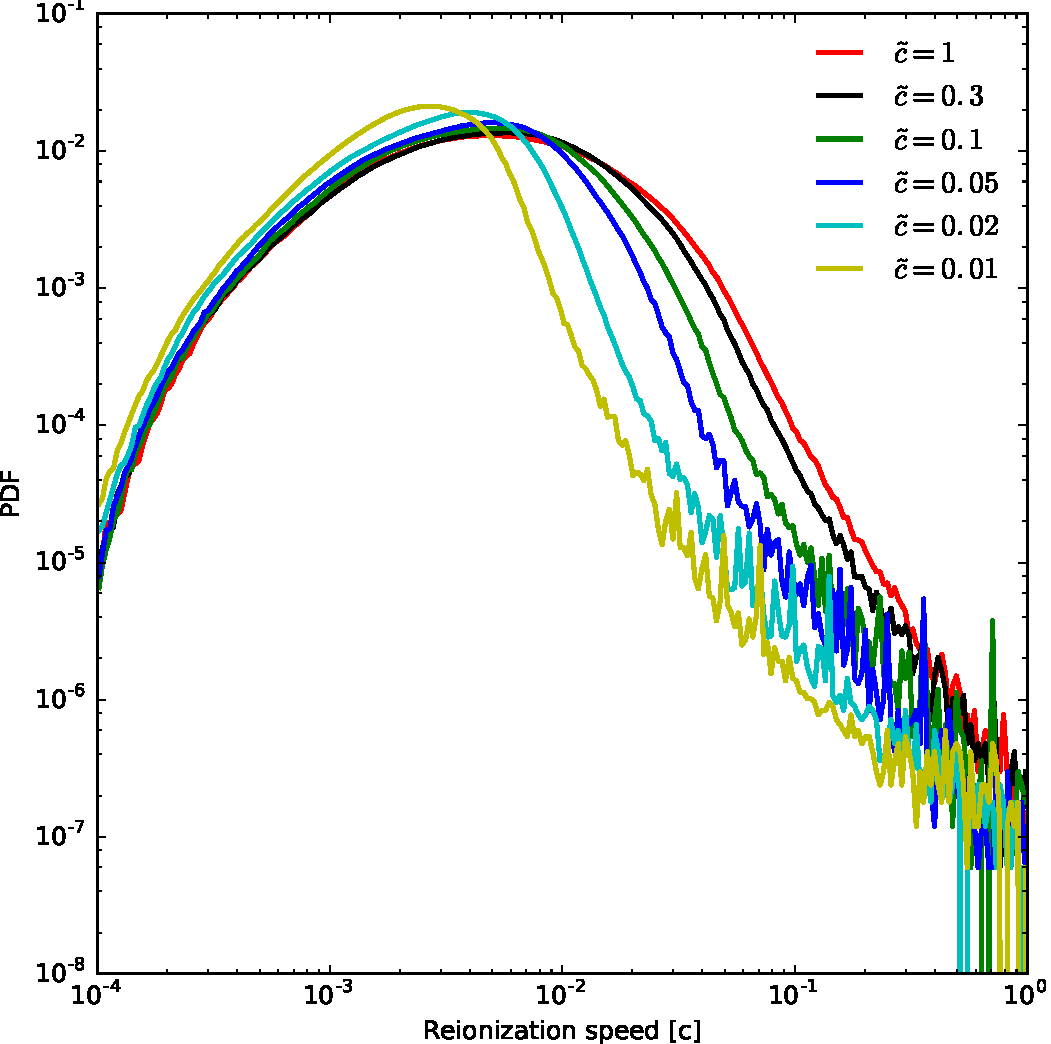
\includegraphics[width=.95\linewidth]{img/04_mapreio/PDF_v_reio.pdf} 
%        \caption[PDF des vitesses de fronts]{Densité de probabilité des vitesses des fronts d'ionisation dans les simulations.
%        La RSLA n’empêche pas de trouver des vitesses de fronts supérieure à la vitesse réduite, mais en réduit la probabilité.
%		\label{fig:pdfv}}
%\end{figure}
%
%La figure \ref{fig:pdfv} présente la densité de probabilité de trouver une valeur de vitesse de front pour différentes \ac{RSLA}.
%On y observe que diminuer la vitesse de la lumière dans la simulation n'interdit pas la présence de front plus rapide que cette vitesse mais en réduit fortement la probabilité.
%Par exemple la courbe jaune correspondant à $\tilde{c}=0.01$, présente une forte décroissance de la probabilité de  trouver une vitesse de  $\tilde{c}=0.01$, mais des vitesses supérieures restent présentes dans le volume.


\begin{figure}
\centering
		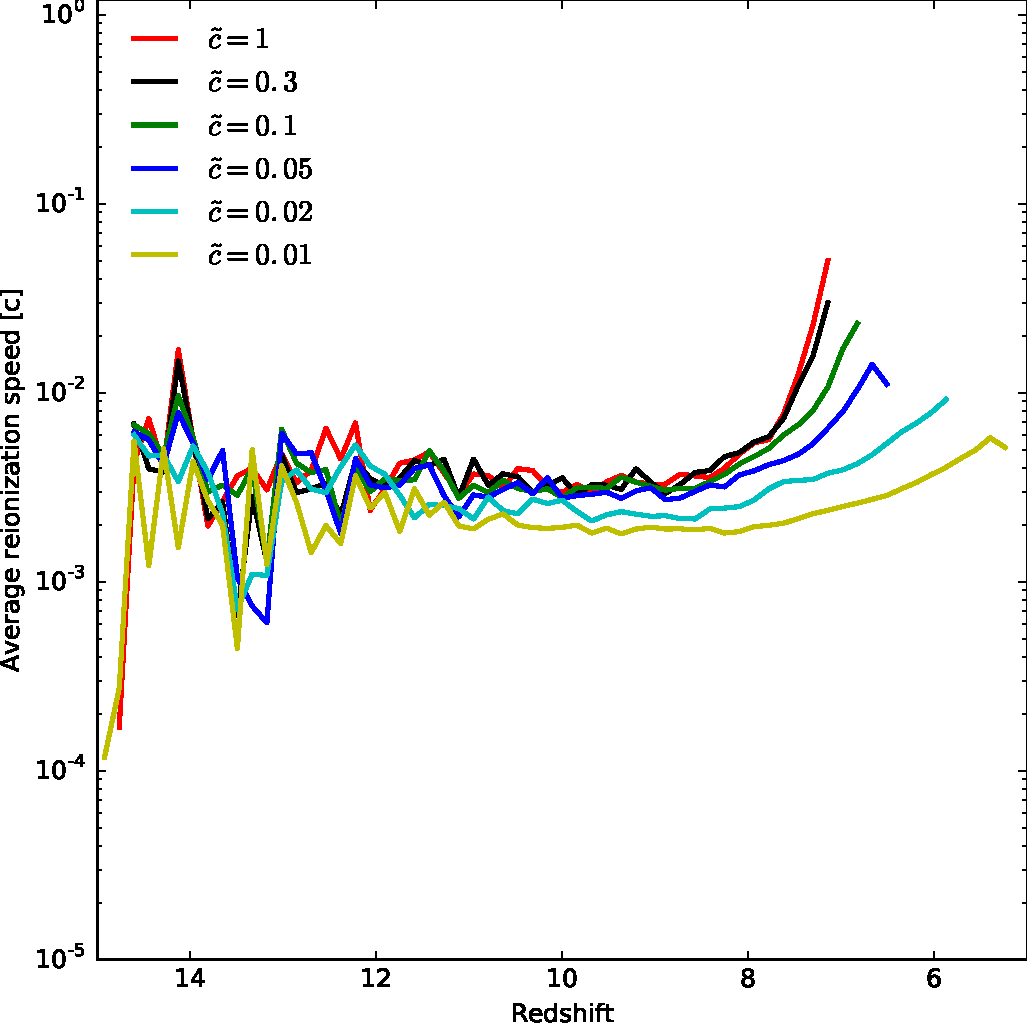
\includegraphics[width=.9\linewidth]{img/04_mapreio/avg_reionization_speed.pdf} 
        \caption[Évolution de la vitesse moyenne des fronts]{Vitesse des fronts d'ionisation en fonction du redshift pour différentes \ac{RSLA}.
        En diminuant $\tilde{c}$, on limite d'abord la seconde phase de la réionisation (l'ionisation des régions sous-denses), puis la première (l'ionisation des régions sur-denses).
        La \ac{RSLA} limite la vitesse moyenne des fronts dans la seconde phase.
        Dans la première phase de la réionisation, la vitesse est quasi constante et seules les valeurs de $\tilde{c} < 5\% $ ont un impact sur la vitesse moyenne.
        }        
 		\label{fig:vreioz_avg}
\end{figure}



\begin{figure}
\centering
        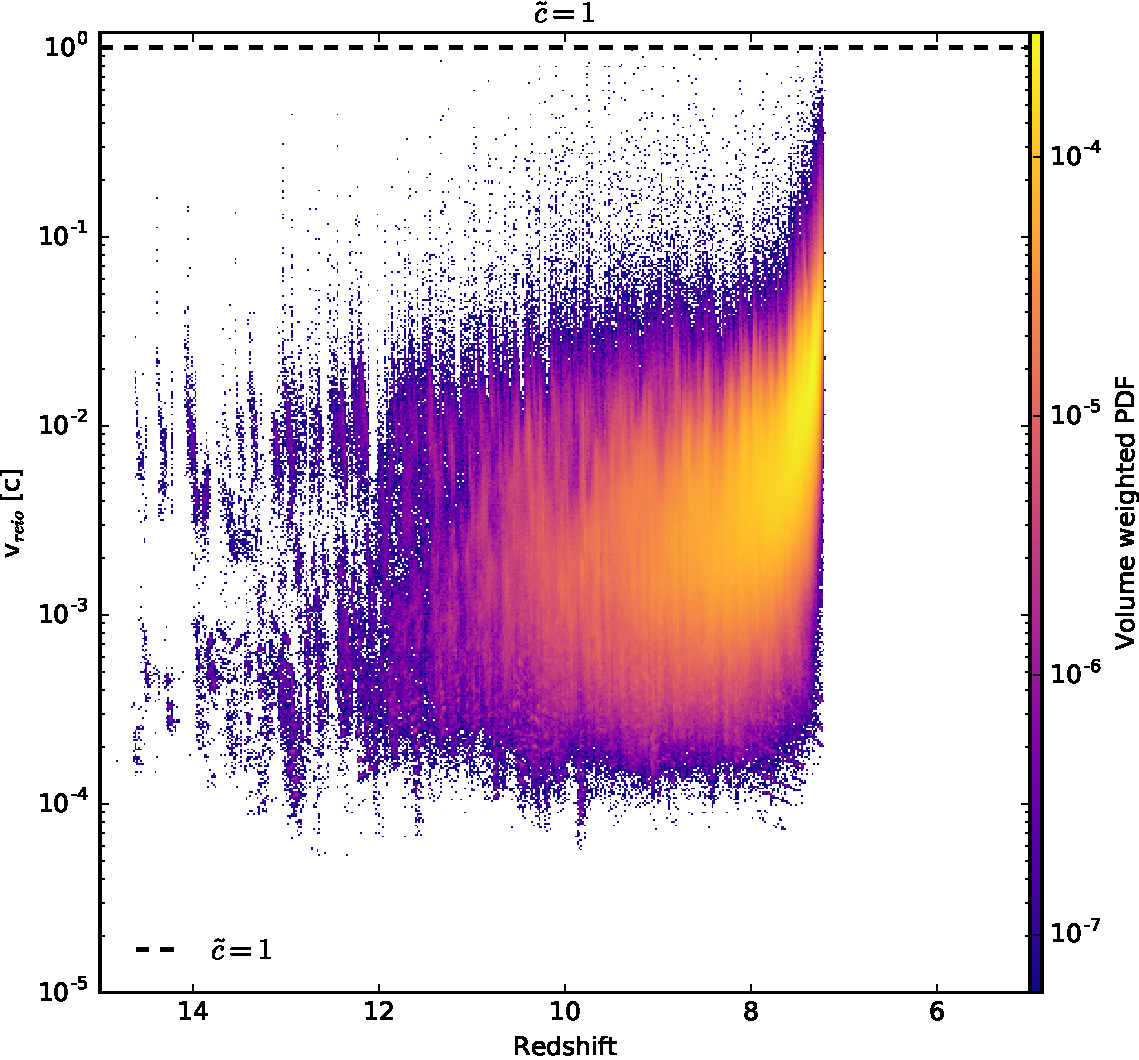
\includegraphics[height=0.3\textheight]{img/04_mapreio/speedreio_z_c1.pdf} 
        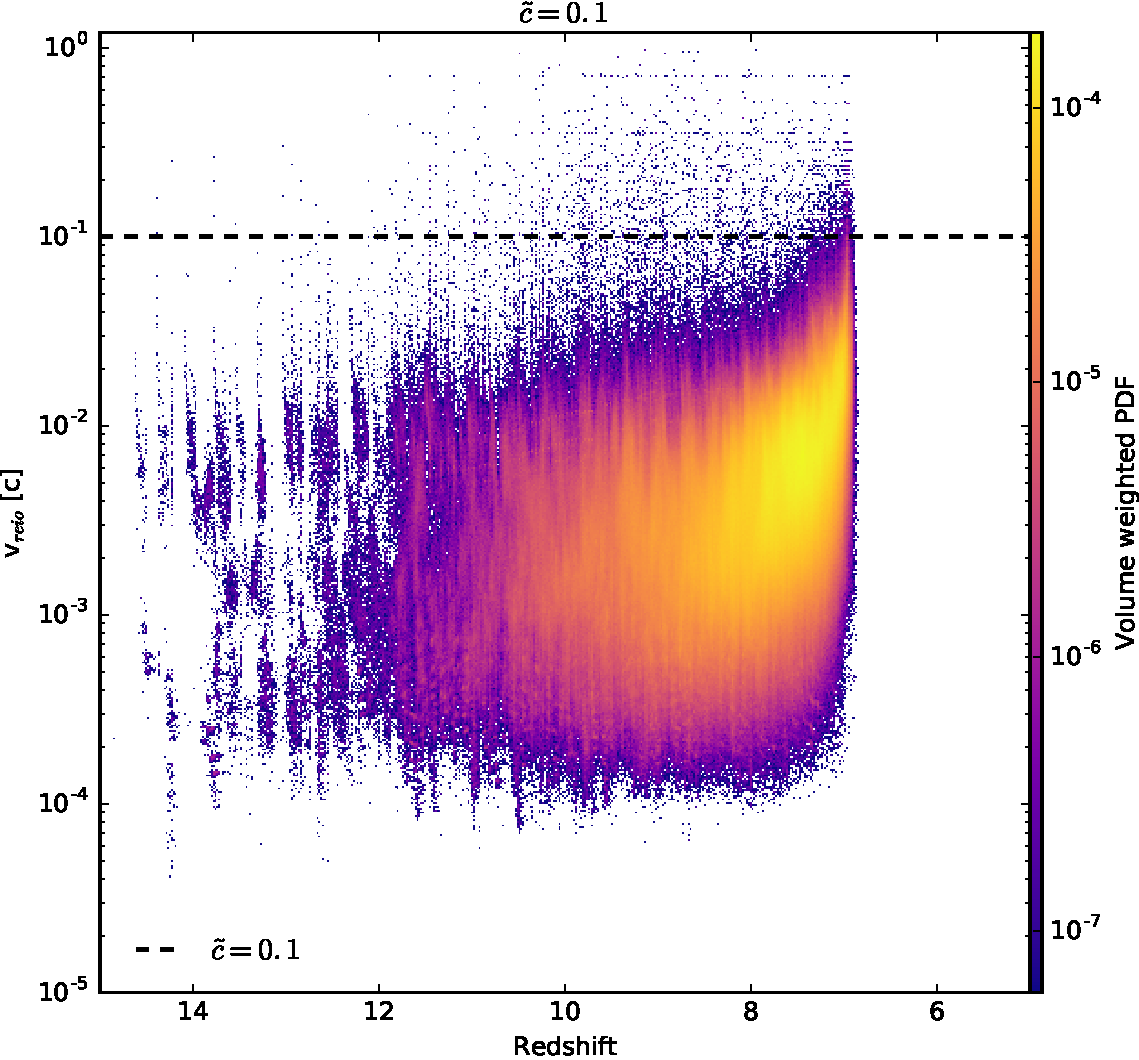
\includegraphics[height=0.3\textheight]{img/04_mapreio/speedreio_z_c01.pdf}
        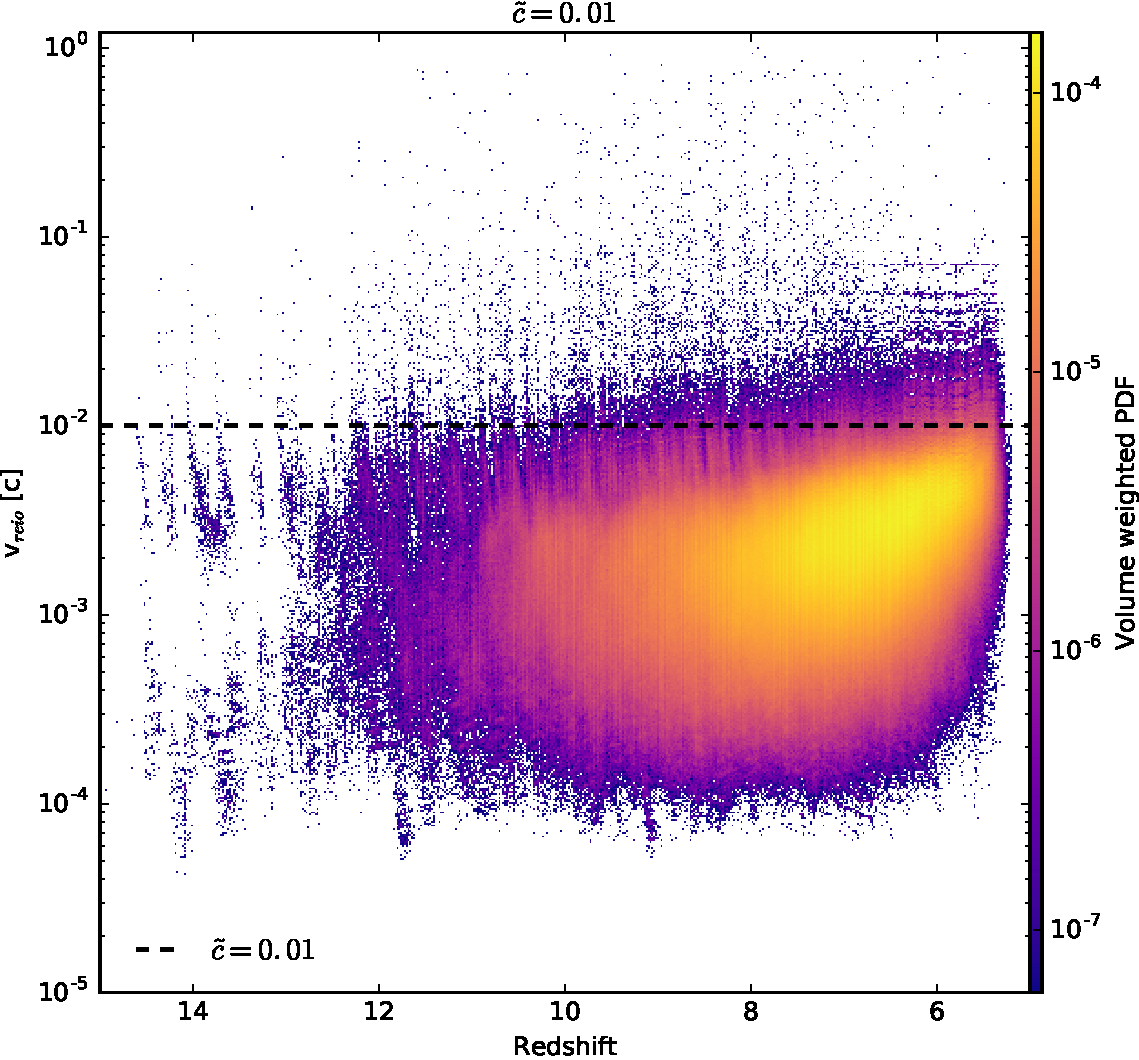
\includegraphics[height=0.3\textheight]{img/04_mapreio/speedreio_z_c001.pdf} 
        \caption[Évolution de la vitesse des fronts - histogrammes]{Vitesse des fronts d'ionisation en fonction du redshift pour différentes \ac{RSLA}.
        En diminuant $\tilde{c}$, on limite d'abord la seconde phase de la réionisation (l'ionisation des zones sous-dense), puis la première (l'ionisation des régions sur-denses).
 		\label{fig:vreioz} }
\end{figure}




\clearpage
\section{Conclusion}

Les carte de redshift de réionisation contiennent une grande quantité d'information et sont des outils essentiels pour étudier la propagation de l'ionisation dans l'\ac{IGM}.
Dans ce chapitre j'ai présenté la méthode de calcul à la volée des cartes de redshift d'ionisation que j'ai implémenté dans EMMA.
A partir de ces cartes j'ai établi une méthode d’estimation de la vitesses des fronts d'ionisation a posteriori.

%En utilisant cette méthode, j'ai montré qu'il existe une corrélation entre la vitesse d'un front et sont accélération: plus un front est rapide, plus il accélère suggérant que la réionisation est un processus exponentiel.
En utilisant cette méthode, j'ai mis en évidence que la réionisation est un processus qui s’exécute en deux temps.
Premièrement une phases où les fronts ont une vitesse quasi constante, suivie d'une seconde phase accélérée.
La première a lieu lorsque le rayonnement travail à sortir des région dense, la seconde phase, lorsque le rayonnement atteint les régions sous-denses et que les bulles percolent.
Dans la seconde phase, les fronts d'ionisations peuvent atteindre une vitesse proche de celle de la lumière.

La \ac{RSLA} n'a pas d'impact sur la \ac{SFH} cosmique et le budget de photon est conservé, mais elle limite la vitesse de propagation des fronts.
Pour les vitesses supérieures à 5\% de la vitesse de la lumière réelle, l'impact ce concentre sur la seconde partie de la réionisation.
Dans le cas ou la vitesse de la lumière réduite est inférieure à 5\% de la vitesse de la lumière réelle, la limitation de vitesse apparaît dès la démarrage et le rayonnement 

On prendra garde, en fonction de ce que l'on cherche à étudier, à l'influence de la \ac{RSLA}.
Dans tout les cas, réduire la vitesse de la lumière à moins de 5\% de se vraie valeur mène à sous estimer la vitesse des fronts, indépendamment du redshift.
A l'inverse, pour les valeur de $\tilde{c} > 0.05$ la vitesse des fronts n'est pas impactée dans la première phase à des redshifts $z>8$, ce qui permet d'étudier la façon dont le rayonnent s’échappe des zones sur-dense sans être biaisé par la \ac{RSLA}.

Enfin une vitesse réduite à 30\% de la valeur réelle présente une évolution quasi similaire à $\tilde{c}=1$ tout en réduisant la coût numérique de la radiation d'un facteur 3.
Cette valeur semble être à privilégiée, plutôt qu'une valeur de $\tilde{c}=0.1$ plus couramment employée.

Le lien entre la vitesse des fronts et la densité de baryon pourrait être explorée plus en détail en conservant en mémoire, en plus de l'instant d'ionisation, la densité de la cellule à cet instant.

Les volumes considérés dans cette étude étant relativement petits, les sources lumineuse et les régions sous-denses ne sont pas entièrement représentées statistiquement.
Dans un volume plus grand, il est possible que les conclusions soient différentes.
Par exemple, comme les régions sous-denses sont sous représentées ici, l'effet de la seconde phase à vitesses élevées risque d'être encore plus important dans des simulations présentant des régions sous-denses plus étendues.

Au final, l'outil de calcul de la vitesse des fronts d'ionisation a été appliqué ici au cas de l'étude de la \ac{RSLA} mais pourrait être utilisée pour tirer des conclusions plus astrophysique.
%Comme une réionisation interne a des conséquences sur la distribution radiale de galaxies satellites \citep{2011MNRAS.417L..93O}
Par exemple, \citep{2011MNRAS.417L..93O} ont montré à l'aide d'un modèle semi analytique, qu'une réionisation rapide est signe d'une réionisation externe et qu'a l'inverse une réionisation plus lente à tendance à signifier une réionisation interne.
%Ils ont également montré que le timing d'ionisation à une influence sur la distribution radiale des satéllite
Ils ont également montré qu'une réionisation interne a des conséquences sur la distribution radiale de galaxies satellites 
Avec la méthode présentée ici, il serait possible de tester cette hypothèse à l'aide de simulations entièrement couplées et d'étudier le lien entre la vitesse des fronts sortant d'une galaxie et le timing de photon-évaporation de ces satellites.

%De plus ils ont montré que lors d'une reionisation interne le timing de réionisation à une influence sur la distribution radiale des satellites.
%À l'aide du calcul de la vitesse des fronts d'ionisation, il serait possible de lier le timing de réionisation des satellites à la vitesse des fronts d'ionisation auxquels ils sont soumis.


%
%En utilisant les simulations présentées dans la prochaine section, il serait également possible d'étudier l'influence de l’environnement cosmologique sur la vitesse de propagation de l'ionisation dans le Groupe Local par exemple et ainsi quantifier la vitesse à la quelle le rayonnement à 



%Réionisation isolée de M31 et MW
%LG pas influencé par Virgo
%Distribution radiale des satélites 


%Cette étude ne porte que sur le cas de solveur radiatif utilisant l'approximation M1 %TODO ref



%Dans cette partie, les fronts d'ionisation atteignent les zones sous-denses et leurs vitesses atteins des valeurs proches de celle de la lumière et si cette dernière est réduite, la vitesse des fronts l'est également.
%
%
%La \ac{RSLA} a une influence sur la propagation de l'ionisation : plus la vitesse de la lumière est élevée dans la simulation, plus le volume réionise rapidement.



